% Options for packages loaded elsewhere
\PassOptionsToPackage{unicode}{hyperref}
\PassOptionsToPackage{hyphens}{url}
%
\documentclass[
]{article}
\usepackage{lmodern}
\usepackage{amssymb,amsmath}
\usepackage{ifxetex,ifluatex}
\ifnum 0\ifxetex 1\fi\ifluatex 1\fi=0 % if pdftex
  \usepackage[T1]{fontenc}
  \usepackage[utf8]{inputenc}
  \usepackage{textcomp} % provide euro and other symbols
\else % if luatex or xetex
  \usepackage{unicode-math}
  \defaultfontfeatures{Scale=MatchLowercase}
  \defaultfontfeatures[\rmfamily]{Ligatures=TeX,Scale=1}
\fi
% Use upquote if available, for straight quotes in verbatim environments
\IfFileExists{upquote.sty}{\usepackage{upquote}}{}
\IfFileExists{microtype.sty}{% use microtype if available
  \usepackage[]{microtype}
  \UseMicrotypeSet[protrusion]{basicmath} % disable protrusion for tt fonts
}{}
\makeatletter
\@ifundefined{KOMAClassName}{% if non-KOMA class
  \IfFileExists{parskip.sty}{%
    \usepackage{parskip}
  }{% else
    \setlength{\parindent}{0pt}
    \setlength{\parskip}{6pt plus 2pt minus 1pt}}
}{% if KOMA class
  \KOMAoptions{parskip=half}}
\makeatother
\usepackage{xcolor}
\IfFileExists{xurl.sty}{\usepackage{xurl}}{} % add URL line breaks if available
\IfFileExists{bookmark.sty}{\usepackage{bookmark}}{\usepackage{hyperref}}
\hypersetup{
  pdftitle={The Influence of Individual Characterisitcs on Public Transportation Planning},
  pdfauthor={Iris Zhong},
  hidelinks,
  pdfcreator={LaTeX via pandoc}}
\urlstyle{same} % disable monospaced font for URLs
\usepackage[margin=1in]{geometry}
\usepackage{color}
\usepackage{fancyvrb}
\newcommand{\VerbBar}{|}
\newcommand{\VERB}{\Verb[commandchars=\\\{\}]}
\DefineVerbatimEnvironment{Highlighting}{Verbatim}{commandchars=\\\{\}}
% Add ',fontsize=\small' for more characters per line
\usepackage{framed}
\definecolor{shadecolor}{RGB}{248,248,248}
\newenvironment{Shaded}{\begin{snugshade}}{\end{snugshade}}
\newcommand{\AlertTok}[1]{\textcolor[rgb]{0.94,0.16,0.16}{#1}}
\newcommand{\AnnotationTok}[1]{\textcolor[rgb]{0.56,0.35,0.01}{\textbf{\textit{#1}}}}
\newcommand{\AttributeTok}[1]{\textcolor[rgb]{0.77,0.63,0.00}{#1}}
\newcommand{\BaseNTok}[1]{\textcolor[rgb]{0.00,0.00,0.81}{#1}}
\newcommand{\BuiltInTok}[1]{#1}
\newcommand{\CharTok}[1]{\textcolor[rgb]{0.31,0.60,0.02}{#1}}
\newcommand{\CommentTok}[1]{\textcolor[rgb]{0.56,0.35,0.01}{\textit{#1}}}
\newcommand{\CommentVarTok}[1]{\textcolor[rgb]{0.56,0.35,0.01}{\textbf{\textit{#1}}}}
\newcommand{\ConstantTok}[1]{\textcolor[rgb]{0.00,0.00,0.00}{#1}}
\newcommand{\ControlFlowTok}[1]{\textcolor[rgb]{0.13,0.29,0.53}{\textbf{#1}}}
\newcommand{\DataTypeTok}[1]{\textcolor[rgb]{0.13,0.29,0.53}{#1}}
\newcommand{\DecValTok}[1]{\textcolor[rgb]{0.00,0.00,0.81}{#1}}
\newcommand{\DocumentationTok}[1]{\textcolor[rgb]{0.56,0.35,0.01}{\textbf{\textit{#1}}}}
\newcommand{\ErrorTok}[1]{\textcolor[rgb]{0.64,0.00,0.00}{\textbf{#1}}}
\newcommand{\ExtensionTok}[1]{#1}
\newcommand{\FloatTok}[1]{\textcolor[rgb]{0.00,0.00,0.81}{#1}}
\newcommand{\FunctionTok}[1]{\textcolor[rgb]{0.00,0.00,0.00}{#1}}
\newcommand{\ImportTok}[1]{#1}
\newcommand{\InformationTok}[1]{\textcolor[rgb]{0.56,0.35,0.01}{\textbf{\textit{#1}}}}
\newcommand{\KeywordTok}[1]{\textcolor[rgb]{0.13,0.29,0.53}{\textbf{#1}}}
\newcommand{\NormalTok}[1]{#1}
\newcommand{\OperatorTok}[1]{\textcolor[rgb]{0.81,0.36,0.00}{\textbf{#1}}}
\newcommand{\OtherTok}[1]{\textcolor[rgb]{0.56,0.35,0.01}{#1}}
\newcommand{\PreprocessorTok}[1]{\textcolor[rgb]{0.56,0.35,0.01}{\textit{#1}}}
\newcommand{\RegionMarkerTok}[1]{#1}
\newcommand{\SpecialCharTok}[1]{\textcolor[rgb]{0.00,0.00,0.00}{#1}}
\newcommand{\SpecialStringTok}[1]{\textcolor[rgb]{0.31,0.60,0.02}{#1}}
\newcommand{\StringTok}[1]{\textcolor[rgb]{0.31,0.60,0.02}{#1}}
\newcommand{\VariableTok}[1]{\textcolor[rgb]{0.00,0.00,0.00}{#1}}
\newcommand{\VerbatimStringTok}[1]{\textcolor[rgb]{0.31,0.60,0.02}{#1}}
\newcommand{\WarningTok}[1]{\textcolor[rgb]{0.56,0.35,0.01}{\textbf{\textit{#1}}}}
\usepackage{graphicx,grffile}
\makeatletter
\def\maxwidth{\ifdim\Gin@nat@width>\linewidth\linewidth\else\Gin@nat@width\fi}
\def\maxheight{\ifdim\Gin@nat@height>\textheight\textheight\else\Gin@nat@height\fi}
\makeatother
% Scale images if necessary, so that they will not overflow the page
% margins by default, and it is still possible to overwrite the defaults
% using explicit options in \includegraphics[width, height, ...]{}
\setkeys{Gin}{width=\maxwidth,height=\maxheight,keepaspectratio}
% Set default figure placement to htbp
\makeatletter
\def\fps@figure{htbp}
\makeatother
\setlength{\emergencystretch}{3em} % prevent overfull lines
\providecommand{\tightlist}{%
  \setlength{\itemsep}{0pt}\setlength{\parskip}{0pt}}
\setcounter{secnumdepth}{5}
\usepackage{booktabs}
\usepackage{setspace}
\doublespacing
\usepackage[labelfont=bf]{caption}
\usepackage{booktabs}
\usepackage{longtable}
\usepackage{array}
\usepackage{multirow}
\usepackage{wrapfig}
\usepackage{float}
\usepackage{colortbl}
\usepackage{pdflscape}
\usepackage{tabu}
\usepackage{threeparttable}
\usepackage{threeparttablex}
\usepackage[normalem]{ulem}
\usepackage{makecell}
\usepackage{xcolor}

\title{The Influence of Individual Characterisitcs on Public Transportation
Planning\thanks{xx}}
\author{Iris Zhong}
\date{}

\begin{document}
\maketitle
\begin{abstract}
xx
\end{abstract}

\begin{verbatim}
## Warning: package 'tidyverse' was built under R version 3.5.3
\end{verbatim}

\begin{verbatim}
## Warning: package 'ggplot2' was built under R version 3.5.3
\end{verbatim}

\begin{verbatim}
## Warning: package 'tibble' was built under R version 3.5.3
\end{verbatim}

\begin{verbatim}
## Warning: package 'tidyr' was built under R version 3.5.3
\end{verbatim}

\begin{verbatim}
## Warning: package 'readr' was built under R version 3.5.3
\end{verbatim}

\begin{verbatim}
## Warning: package 'purrr' was built under R version 3.5.3
\end{verbatim}

\begin{verbatim}
## Warning: package 'dplyr' was built under R version 3.5.3
\end{verbatim}

\begin{verbatim}
## Warning: package 'stringr' was built under R version 3.5.3
\end{verbatim}

\begin{verbatim}
## Warning: package 'forcats' was built under R version 3.5.3
\end{verbatim}

\begin{verbatim}
## Warning: package 'lubridate' was built under R version 3.5.3
\end{verbatim}

\begin{verbatim}
## Warning: package 'stargazer' was built under R version 3.5.2
\end{verbatim}

\hypertarget{literature-review}{%
\section{Literature Review}\label{literature-review}}

Allen et al.~(2016) study the reasoning of the failure of a referendum
on a congestion charging scheme in Edinburgh. Instead of using direct
voting data, they conduct a survey after the referendum, which allows
them to ask more specific questions. Researchers can gain detailed data
by surveying, because the unit of measurement is each individual;
however, a possible disadvantage of surveying is that respondents who
turn in the questionnaire tend to have stronger attitudes towards the
proposal, generating sampling bias. They conclude that people who use
cars as the primary transportation mean, demonstrate a misconception of
the pricing plan, or question the effectiveness of the scheme at
reducing congestion are more likely to oppose it. Their findings can
give insights to the similar failure in the Gwinnett referendum. Voters
against the proposal could be those who rarely use public transportation
and those who are not convinced by the effectiveness of expanding public
transit in alleviating the traffic.

Another crucial factor is the accessibility of the proposed transit
system. Kinsey et al.~(2010) examine the relationship between the
distance to the scheduled railway station and voter turnout by studying
the Seattle monorail referendum. They introduce the concept of diffused
and concentrated benefit/cost. People who live far from the monorail
enjoy the diffused benefit of less traffic congestion, and bear the
diffused cost of increased tax. People living close to the rail
experience the same diffused benefit and cost, but they also gain the
concentrated benefit of easily accessing the public good. Finally, those
who live very close to the railway have the same benefits and costs, but
they also face the concentrated cost such as inconvenience during
construction. Since ``people are more strongly motivated to avoid losses
than to approach gains,'' they expect a higher turnout rate in farther
places with votes for ``no,'' which is verified from their analyses.
Besides distance, they also find out precincts with a higher percentage
of people of lower socioeconomic status or young people have a lower
turnout rate. Interestingly, there is a significant interaction between
partisanship and distance, which would be also tested in my study. In
essence, the effect of distance on turnout is weakened by partisanship,
and vanishes beyond a threshold of distance. Even though my dependent
variable is voters' responses rather than turnout, it can be inferred
from Kinsey et al.'s findings that people farther away from the transit
system would vote against the referendum more. However, the relationship
might be non-linear and requires some form of transformation. Regarding
the methods, they utilize the spatial lag model to correct for
autocorrelation, which is proper to use in my project as well since both
studies use precinct-level data.

\hypertarget{background}{%
\section{Background}\label{background}}

current transportation future plan referendum

\hypertarget{data-methods}{%
\section{Data \& Methods}\label{data-methods}}

\hypertarget{conceptual-model}{%
\subsection{Conceptual model}\label{conceptual-model}}

\hypertarget{data}{%
\subsection{Data}\label{data}}

\begin{table}
\centering
\caption{Variable definitions}
\label{variableDefinitions}
\begin{tabular}{ll}
\hline
\hline
Variable name      & Description                                   \\
\hline
GEOID          & The geographic identifier of the census tract                 \\
medage        & The median age of the population in the tract               \\
medincome        & The median income of the population in the tract               \\
white\_pct           & The percentage of white population in the tract      \\
public\_pct          & The percentage of people who go to work by public transportation (excluding taxi or cab)      \\
time\_pct           & The percentage of people who travel more than an hour to work      \\
trump\_pct          & The estimated percentage of votes for Donald Trump in that tract      \\
voter\_turnout  & The estimated percentage of voters who voted in this referendum in the tract \\
yes\_pct           & The estimated percentage of voters who voted yes in this referendum in the tract      \\
plan\_yes          & Whether the tract is covered by short-range plan. 1 stands for yes, 0 stands for no      \\
current\_yes          & Whether the tract is covered by the existing public transportation. 1 stands for yes, 0 stands for no      \\
\hline
\end{tabular}
\end{table}

\begin{itemize}
\tightlist
\item
  \textbf{GEOID:} The geographic identifier of the census tract.\\
\item
  \textbf{medage:} The median age of the population in the tract.
\item
  \textbf{medincome:} The median income of the population in the tract.
\item
  \textbf{white\_pct:} The percentage of white population in the tract.
\item
  \textbf{public\_pct:} The percentage of people who go to work by
  public transportation (excluding taxi or cab).\\
\item
  \textbf{time\_pct:} The percentage of people who travel more than an
  hour to work.\\
\item
  \textbf{trump\_pct:} The estimated percentage of votes for Donald
  Trump in that tract.
\item
  \textbf{voter\_turnout:} The estimated percentage of voters who voted
  in this referendum in the tract.
\item
  \textbf{yes\_pct:} The estimated percentage of voters who voted yes in
  this referendum in the tract.
\item
  \textbf{plan\_yes:} Whether the tract is covered by the public
  transportation planned in the short-range (Y2020 -- 2025), defined by
  whether any transportation is available within 500 meters. 1 stands
  for yes, 0 stands for no.\\
\item
  \textbf{current\_yes:} Whether the tract is covered by the existing
  public transportation, defined by whether any transportation is
  available within 500 meters. 1 stands for yes, 0 stands for no.
\end{itemize}

\hypertarget{results}{%
\section{Results}\label{results}}

model 1: all variables, no interaction, linear

\begin{Shaded}
\begin{Highlighting}[]
\KeywordTok{load}\NormalTok{(}\StringTok{"processed_data/analysis_data.RData"}\NormalTok{)}
\NormalTok{mod1 <-}\StringTok{ }\KeywordTok{lm}\NormalTok{(}\DataTypeTok{data =}\NormalTok{ final_data, yes_pct }\OperatorTok{~}\StringTok{ }\NormalTok{medage }\OperatorTok{+}\StringTok{ }\NormalTok{medincome }\OperatorTok{+}\StringTok{ }\NormalTok{white_pct }\OperatorTok{+}\StringTok{ }\NormalTok{public_pct }\OperatorTok{+}\StringTok{ }\NormalTok{time_pct }\OperatorTok{+}\StringTok{ }\NormalTok{trump_pct }\OperatorTok{+}\StringTok{ }\NormalTok{voter_turnout }\OperatorTok{+}\StringTok{ }\NormalTok{plan_yes }\OperatorTok{+}\StringTok{ }\NormalTok{current_yes)}
\KeywordTok{summary}\NormalTok{(mod1)}
\end{Highlighting}
\end{Shaded}

Call: lm(formula = yes\_pct \textasciitilde{} medage + medincome +
white\_pct + public\_pct + time\_pct + trump\_pct + voter\_turnout +
plan\_yes + current\_yes, data = final\_data)

Residuals: Min 1Q Median 3Q Max -0.103384 -0.031723 -0.004037 0.030238
0.101018

Coefficients: Estimate Std. Error t value
Pr(\textgreater\textbar t\textbar)\\
(Intercept) 8.016e-01 4.677e-02 17.138 \textless{} 2e-16 \textbf{\emph{
medage 2.733e-03 1.477e-03 1.851 0.067054 .\\
medincome 1.458e-07 2.914e-07 0.500 0.617850\\
white\_pct 1.177e-01 5.285e-02 2.226 0.028162 }\\
public\_pct 8.393e-01 3.355e-01 2.501 0.013946 *\\
time\_pct -3.029e-01 9.013e-02 -3.361 0.001090 } trump\_pct -8.884e-01
5.680e-02 -15.640 \textless{} 2e-16 \textbf{\emph{ voter\_turnout
-3.285e-01 1.257e-01 -2.613 0.010323 }\\
plan\_yes1 -2.967e-02 1.153e-02 -2.573 0.011511 *\\
current\_yes1 4.627e-02 1.209e-02 3.825 0.000224 }* --- Signif. codes: 0
`\emph{\textbf{' 0.001 '}' 0.01 '}' 0.05 `.' 0.1 ' ' 1

Residual standard error: 0.04185 on 103 degrees of freedom Multiple
R-squared: 0.917, Adjusted R-squared: 0.9098 F-statistic: 126.5 on 9 and
103 DF, p-value: \textless{} 2.2e-16

model 1 assumption checking

\begin{Shaded}
\begin{Highlighting}[]
\KeywordTok{plot}\NormalTok{(}\KeywordTok{predict}\NormalTok{(mod1),}\KeywordTok{resid}\NormalTok{(mod1),}\DataTypeTok{col=}\StringTok{"midnightblue"}\NormalTok{,}\DataTypeTok{pch=}\DecValTok{18}\NormalTok{,}\DataTypeTok{main=}\StringTok{"Residual plot - Model 1"}\NormalTok{)}
\KeywordTok{abline}\NormalTok{(}\DecValTok{0}\NormalTok{,}\DecValTok{0}\NormalTok{,}\DataTypeTok{col=}\StringTok{"red"}\NormalTok{)}
\end{Highlighting}
\end{Shaded}

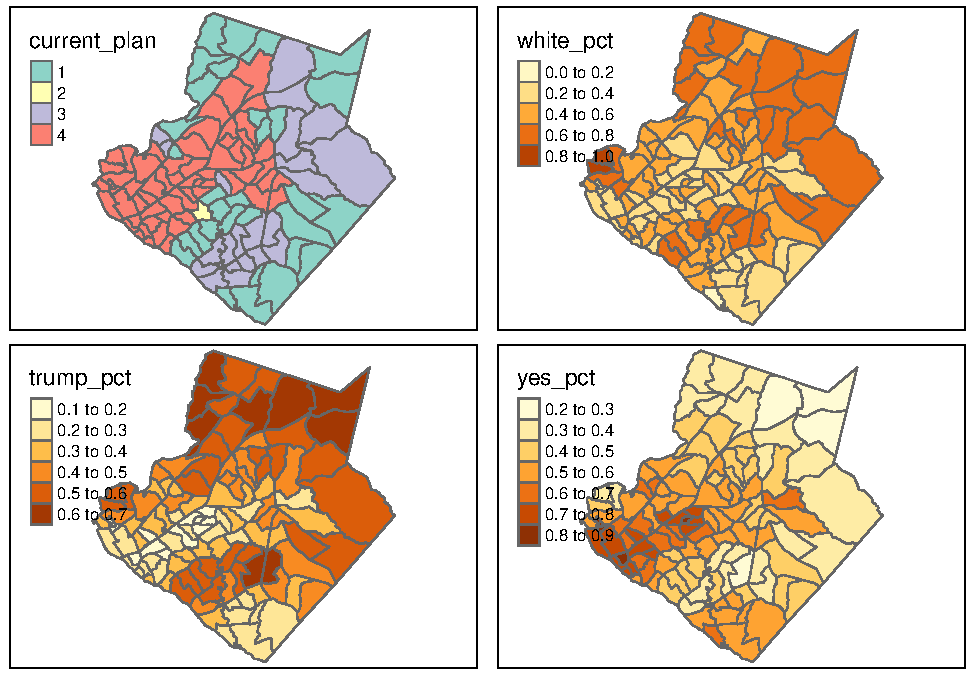
\includegraphics{Zhong_paper_files/figure-latex/unnamed-chunk-2-1.pdf}

collinearity:

\begin{Shaded}
\begin{Highlighting}[]
\KeywordTok{library}\NormalTok{(car)}
\end{Highlighting}
\end{Shaded}

\begin{verbatim}
## Warning: package 'car' was built under R version 3.5.3
\end{verbatim}

\begin{verbatim}
## Loading required package: carData
\end{verbatim}

\begin{verbatim}
## Warning: package 'carData' was built under R version 3.5.3
\end{verbatim}

\begin{verbatim}
## 
## Attaching package: 'car'
\end{verbatim}

\begin{verbatim}
## The following object is masked from 'package:dplyr':
## 
##     recode
\end{verbatim}

\begin{verbatim}
## The following object is masked from 'package:purrr':
## 
##     some
\end{verbatim}

\begin{Shaded}
\begin{Highlighting}[]
\KeywordTok{vif}\NormalTok{(mod1)}
\end{Highlighting}
\end{Shaded}

\begin{verbatim}
   medage     medincome     white_pct    public_pct      time_pct 
 2.920936      3.221504      3.863617      1.151309      1.559837 
trump_pct voter_turnout      plan_yes   current_yes 
 4.512575      3.368751      1.741403      2.350032 
\end{verbatim}

all below 5: good, no collinearity problem

model 2: all variables, no interaction, logistic

\begin{Shaded}
\begin{Highlighting}[]
\NormalTok{mod2 <-}\StringTok{ }\KeywordTok{glm}\NormalTok{(}\DataTypeTok{data =}\NormalTok{ final_data, yes_pct }\OperatorTok{~}\StringTok{ }\NormalTok{medage }\OperatorTok{+}\StringTok{ }\NormalTok{medincome }\OperatorTok{+}\StringTok{ }\NormalTok{white_pct }\OperatorTok{+}\StringTok{ }\NormalTok{public_pct }\OperatorTok{+}\StringTok{ }\NormalTok{time_pct }\OperatorTok{+}\StringTok{ }\NormalTok{trump_pct }\OperatorTok{+}\StringTok{ }\NormalTok{voter_turnout }\OperatorTok{+}\StringTok{ }\NormalTok{plan_yes }\OperatorTok{+}\StringTok{ }\NormalTok{current_yes, }\DataTypeTok{family =} \StringTok{"binomial"}\NormalTok{)}
\end{Highlighting}
\end{Shaded}

\begin{verbatim}
## Warning in eval(family$initialize): non-integer #successes in a binomial glm!
\end{verbatim}

\begin{Shaded}
\begin{Highlighting}[]
\KeywordTok{summary}\NormalTok{(mod2)}
\end{Highlighting}
\end{Shaded}

Call: glm(formula = yes\_pct \textasciitilde{} medage + medincome +
white\_pct + public\_pct + time\_pct + trump\_pct + voter\_turnout +
plan\_yes + current\_yes, family = ``binomial'', data = final\_data)

Deviance Residuals: Min 1Q Median 3Q Max\\
-0.224114 -0.065598 -0.003135 0.067243 0.206940

Coefficients: Estimate Std. Error z value
Pr(\textgreater\textbar z\textbar) (Intercept) 1.315e+00 2.311e+00 0.569
0.569 medage 1.068e-02 7.223e-02 0.148 0.882 medincome 6.880e-07
1.432e-05 0.048 0.962 white\_pct 5.666e-01 2.627e+00 0.216 0.829
public\_pct 3.642e+00 1.706e+01 0.213 0.831 time\_pct -1.376e+00
4.462e+00 -0.308 0.758 trump\_pct -3.790e+00 2.839e+00 -1.335 0.182
voter\_turnout -1.453e+00 6.216e+00 -0.234 0.815 plan\_yes1 -1.276e-01
5.671e-01 -0.225 0.822 current\_yes1 1.891e-01 5.911e-01 0.320 0.749

(Dispersion parameter for binomial family taken to be 1)

\begin{verbatim}
Null deviance: 9.05063  on 112  degrees of freedom
\end{verbatim}

Residual deviance: 0.83282 on 103 degrees of freedom AIC: 133.92

Number of Fisher Scoring iterations: 4

model 3: all variables, no interaction, some transformation, linear

step 1: find the skewed variables

\begin{Shaded}
\begin{Highlighting}[]
\KeywordTok{library}\NormalTok{(dlookr)}
\end{Highlighting}
\end{Shaded}

\begin{verbatim}
## Warning: package 'dlookr' was built under R version 3.5.3
\end{verbatim}

\begin{verbatim}
## Loading required package: mice
\end{verbatim}

\begin{verbatim}
## Warning: package 'mice' was built under R version 3.5.3
\end{verbatim}

\begin{verbatim}
## 
## Attaching package: 'mice'
\end{verbatim}

\begin{verbatim}
## The following objects are masked from 'package:base':
## 
##     cbind, rbind
\end{verbatim}

\begin{verbatim}
## 
## Attaching package: 'dlookr'
\end{verbatim}

\begin{verbatim}
## The following object is masked from 'package:base':
## 
##     transform
\end{verbatim}

\begin{Shaded}
\begin{Highlighting}[]
\KeywordTok{find_skewness}\NormalTok{(final_data)}
\end{Highlighting}
\end{Shaded}

{[}1{]} 3 5 8

medincome, public\_pct, voter\_turnout

step 2: transform them

\begin{Shaded}
\begin{Highlighting}[]
\NormalTok{data_tf <-}\StringTok{ }\NormalTok{final_data }\OperatorTok
\StringTok{   }\KeywordTok{mutate}\NormalTok{(}\DataTypeTok{medincome =} \KeywordTok{log}\NormalTok{(medincome),}
          \DataTypeTok{public_pct =} \KeywordTok{log}\NormalTok{(public_pct }\OperatorTok{+}\StringTok{ }\FloatTok{0.01}\NormalTok{),}
          \DataTypeTok{voter_turnout =}\NormalTok{ (voter_turnout)}\OperatorTok{^}\FloatTok{0.5}\NormalTok{)}
\KeywordTok{find_skewness}\NormalTok{(data_tf)}
\end{Highlighting}
\end{Shaded}

integer(0)

step 3: model them

\begin{Shaded}
\begin{Highlighting}[]
\NormalTok{mod3 <-}\StringTok{ }\KeywordTok{lm}\NormalTok{(}\DataTypeTok{data =}\NormalTok{ data_tf, yes_pct }\OperatorTok{~}\StringTok{ }\NormalTok{medage }\OperatorTok{+}\StringTok{ }\NormalTok{medincome }\OperatorTok{+}\StringTok{ }\NormalTok{white_pct }\OperatorTok{+}\StringTok{ }\NormalTok{public_pct }\OperatorTok{+}\StringTok{ }\NormalTok{time_pct }\OperatorTok{+}\StringTok{ }\NormalTok{trump_pct }\OperatorTok{+}\StringTok{ }\NormalTok{voter_turnout }\OperatorTok{+}\StringTok{ }\NormalTok{plan_yes }\OperatorTok{+}\StringTok{ }\NormalTok{current_yes)}
\KeywordTok{summary}\NormalTok{(mod3)}
\end{Highlighting}
\end{Shaded}

Call: lm(formula = yes\_pct \textasciitilde{} medage + medincome +
white\_pct + public\_pct + time\_pct + trump\_pct + voter\_turnout +
plan\_yes + current\_yes, data = data\_tf)

Residuals: Min 1Q Median 3Q Max -0.099662 -0.030760 -0.004331 0.027626
0.097867

Coefficients: Estimate Std. Error t value
Pr(\textgreater\textbar t\textbar)\\
(Intercept) 1.022033 0.217430 4.701 8.07e-06 \textbf{\emph{ medage
0.003595 0.001506 2.386 0.01884 }\\
medincome -0.007268 0.022156 -0.328 0.74356\\
white\_pct 0.119648 0.050332 2.377 0.01929 *\\
public\_pct 0.022875 0.008179 2.797 0.00616 } time\_pct -0.279306
0.089340 -3.126 0.00230 ** trump\_pct -0.859270 0.058269 -14.747
\textless{} 2e-16 \emph{\textbf{ voter\_turnout -0.321784 0.103026
-3.123 0.00232 } plan\_yes1 -0.031542 0.011317 -2.787 0.00633 \textbf{
current\_yes1 0.045541 0.011848 3.844 0.00021 }} --- Signif. codes: 0
`\emph{\textbf{' 0.001 '}' 0.01 '}' 0.05 `.' 0.1 ' ' 1

Residual standard error: 0.04112 on 103 degrees of freedom Multiple
R-squared: 0.9199, Adjusted R-squared: 0.9129 F-statistic: 131.4 on 9
and 103 DF, p-value: \textless{} 2.2e-16

model 3 assumption checking

\begin{Shaded}
\begin{Highlighting}[]
\KeywordTok{plot}\NormalTok{(}\KeywordTok{predict}\NormalTok{(mod3),}\KeywordTok{resid}\NormalTok{(mod3),}\DataTypeTok{col=}\StringTok{"midnightblue"}\NormalTok{,}\DataTypeTok{pch=}\DecValTok{18}\NormalTok{,}\DataTypeTok{main=}\StringTok{"Residual plot - Model 3"}\NormalTok{)}
\KeywordTok{abline}\NormalTok{(}\DecValTok{0}\NormalTok{,}\DecValTok{0}\NormalTok{,}\DataTypeTok{col=}\StringTok{"red"}\NormalTok{)}
\end{Highlighting}
\end{Shaded}

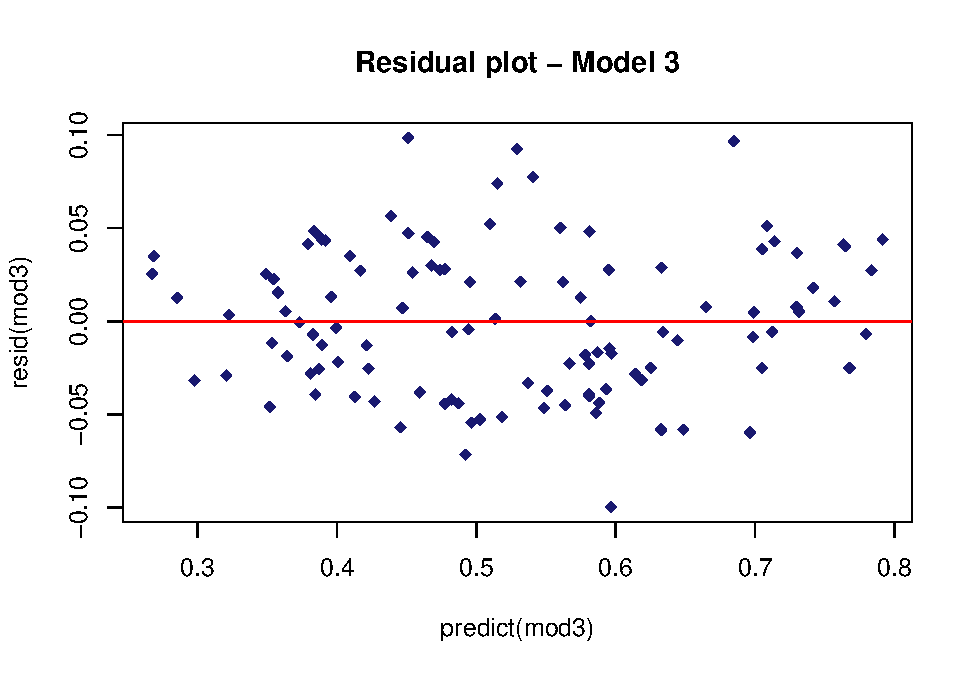
\includegraphics{Zhong_paper_files/figure-latex/unnamed-chunk-8-1.pdf}

collinearity:

\begin{Shaded}
\begin{Highlighting}[]
\KeywordTok{vif}\NormalTok{(mod3)}
\end{Highlighting}
\end{Shaded}

\begin{verbatim}
   medage     medincome     white_pct    public_pct      time_pct 
 3.149466      3.713809      3.629803      1.133155      1.587723 
trump_pct voter_turnout      plan_yes   current_yes 
 4.919508      3.621155      1.737295      2.336190 
\end{verbatim}

all below 5: no collinearity

model 4: all variables, interaction, no transformation, linear

\begin{Shaded}
\begin{Highlighting}[]
\NormalTok{mod4 <-}\StringTok{ }\KeywordTok{lm}\NormalTok{(}\DataTypeTok{data =}\NormalTok{ final_data, yes_pct }\OperatorTok{~}\StringTok{ }\NormalTok{medage }\OperatorTok{+}\StringTok{ }\NormalTok{medincome }\OperatorTok{+}\StringTok{ }\NormalTok{white_pct }\OperatorTok{+}\StringTok{ }\NormalTok{public_pct }\OperatorTok{+}\StringTok{ }\NormalTok{time_pct }\OperatorTok{+}\StringTok{ }\NormalTok{trump_pct }\OperatorTok{+}\StringTok{ }\NormalTok{voter_turnout }\OperatorTok{+}\StringTok{ }\NormalTok{plan_yes }\OperatorTok{*}\StringTok{ }\NormalTok{current_yes)}
\KeywordTok{summary}\NormalTok{(mod4)}
\end{Highlighting}
\end{Shaded}

Call: lm(formula = yes\_pct \textasciitilde{} medage + medincome +
white\_pct + public\_pct + time\_pct + trump\_pct + voter\_turnout +
plan\_yes * current\_yes, data = final\_data)

Residuals: Min 1Q Median 3Q Max -0.103714 -0.032077 -0.002399 0.030226
0.101740

Coefficients: Estimate Std. Error t value
Pr(\textgreater\textbar t\textbar)\\
(Intercept) 8.041e-01 4.707e-02 17.085 \textless{} 2e-16 \textbf{\emph{
medage 2.738e-03 1.481e-03 1.849 0.06739 .\\
medincome 1.326e-07 2.930e-07 0.453 0.65183\\
white\_pct 1.143e-01 5.326e-02 2.147 0.03420 }\\
public\_pct 8.173e-01 3.382e-01 2.417 0.01743 *\\
time\_pct -3.057e-01 9.048e-02 -3.378 0.00103 } trump\_pct -8.859e-01
5.709e-02 -15.517 \textless{} 2e-16 \textbf{\emph{ voter\_turnout
-3.257e-01 1.262e-01 -2.582 0.01125 }\\
plan\_yes1 -3.176e-02 1.201e-02 -2.645 0.00945 } current\_yes1 1.888e-02
4.399e-02 0.429 0.66866\\
plan\_yes1:current\_yes1 2.899e-02 4.476e-02 0.648 0.51864\\
--- Signif. codes: 0 `\emph{\textbf{' 0.001 '}' 0.01 '}' 0.05 `.' 0.1 '
' 1

Residual standard error: 0.04197 on 102 degrees of freedom Multiple
R-squared: 0.9174, Adjusted R-squared: 0.9093 F-statistic: 113.2 on 10
and 102 DF, p-value: \textless{} 2.2e-16

\begin{Shaded}
\begin{Highlighting}[]
\KeywordTok{anova}\NormalTok{(mod1,mod4)}
\end{Highlighting}
\end{Shaded}

Analysis of Variance Table

Model 1: yes\_pct \textasciitilde{} medage + medincome + white\_pct +
public\_pct + time\_pct + trump\_pct + voter\_turnout + plan\_yes +
current\_yes Model 2: yes\_pct \textasciitilde{} medage + medincome +
white\_pct + public\_pct + time\_pct + trump\_pct + voter\_turnout +
plan\_yes * current\_yes Res.Df RSS Df Sum of Sq F Pr(\textgreater F) 1
103 0.18044\\
2 102 0.17970 1 0.00073903 0.4195 0.5186

Model w/ interaction doesn't differ significantly from the one w/o
interaction.

\end{document}
